\documentclass[11pt]{article}

\usepackage[margin=1in]{geometry}
\usepackage{amsmath,amssymb,amsthm}
\usepackage{booktabs}
\usepackage{graphicx}
\usepackage{xcolor}
\usepackage{multirow}
\usepackage{hyperref}
\usepackage[numbers,sort&compress]{natbib}
\usepackage{setspace}
\doublespacing
\usepackage{lineno}
\linenumbers

\newtheorem{proposition}{Proposition}

\renewcommand{\arraystretch}{1.3}
\setlength{\textfloatsep}{12pt plus 2pt minus 2pt}
\setlength{\intextsep}{10pt plus 2pt minus 2pt}
\setlength{\abovecaptionskip}{8pt}
\setlength{\belowcaptionskip}{4pt}

\title{Site-level rates and site-level coefficients estimate different\\
quantities: a record-level benchmark for federated analysis\\
of COVID-19 surveillance data}

% corresponding-author contact details, kept out of tracked source
\IfFileExists{title_contact.tex}{\input{title_contact}}{}
\providecommand{\corrcontact}{}

\author{Elliot Tower, M.S.\\
\textit{Independent Researcher}\\[6pt]
\textbf{Corresponding author:}\\
Elliot Tower\\
Email: \texttt{elliot@elliottower.ai}\\
\corrcontact
\textbf{Word count:} 3320 (excluding title page, abstract, references,
figures and tables)}

\date{}

\begin{document}
\maketitle

\begin{abstract}
\noindent\textbf{Objective:}
Federated networks share site-level rates or coefficients from
site-level models, and treat these as interchangeable.  A regression
across site rates absorbs between-site differences that track the
regressor, so it need not recover the within-site association a
coefficient estimates.  We tested whether the two agree.

\noindent\textbf{Materials and Methods:}
We analyzed 3\,993\,464 confirmed COVID-19 case records from Mexico's
surveillance system, 32 treating-unit states.  The observed
ecological slope regressed state case fatality on the share aged 70 or
older.  The model-implied slope averaged record-level logistic
predictions within each state and regressed those on the same share.  Their difference is the
ecological discrepancy.  We varied the
record-level model across six prespecified specifications and the
site definition across residence state, sector, municipality, and a
random partition holding each state's size and elderly count fixed.

\noindent\textbf{Results:}
Under the prespecified three-covariate model, observed and
model-implied slopes were 1.31 and 0.45 percentage points of case
fatality per point of elderly share (difference 0.86; bootstrap 95\% CI
0.50--1.30).  The difference fell as adjustment increased but remained
0.59 (0.21--1.07) under the richest specification.  On matched records it
was 0.47 across municipalities against 1.01 across states of
residence, and 0.00 under the random partition, by construction.  Aligned one-stage and two-stage estimators
agreed to 0.0007 in the log odds ratio.

\noindent\textbf{Discussion:}
The discrepancy is defined relative to a specified record-level model
and does not identify a contextual effect.

\noindent\textbf{Conclusion:}
Networks sharing rates should name the record-level model their inference
assumes, and share coefficients where a record-level
association is the target.
\end{abstract}

\noindent\textbf{Keywords:} ecological fallacy; multicenter studies; data aggregation;
electronic health records; COVID-19


\section{Background and Significance}

Federated networks are central infrastructure for multi-site clinical
research: ENACT/ACT across the CTSA consortium
\cite{visweswaran2018act}, OHDSI across a common data model
\cite{hripcsak2015ohdsi}, TriNetX across more than 20 countries
\cite{trinetx2024}, and PCORnet across partner networks serving over
47 million patients \cite{fleurence2014pcornet}.  These networks share
different objects, and the ecological fallacy
\cite{robinson1950ecological} arises in the subset of arrangements
where a relationship among site rates is read as an association among
patients: rate and prevalence dashboards, consortia that pool aggregate
counts, and any analysis regressing site rates on site composition.
Networks that fit local models and pool coefficients are not exposed in
the same way, which Table~\ref{tab:estimators} bears out.  The
mechanisms of the fallacy are
well understood \cite{greenland1992ecological,greenland2001ecologic}
and formal frameworks for ecological inference exist
\cite{king1997ecological,wakefield2003ecological,wakefield2008ecologic},
but how far a working federated analysis departs from the
record-level association it is read as estimating has rarely been
measured on data where both can be computed.  Between-site differences
between observed and predicted outcomes are studied as calibration in
multicenter prediction research
\cite{vancalster2019calibration,wynants2018clustering}.  The quantity
measured here is a projection of those differences onto one site-level
covariate, on the sites the record-level model was fitted on rather
than on new centers.

What a network shares is not one choice but several, and they do not
preserve the same thing.  A network may share site-level rates and
prevalences, or coefficients from a model each site fits locally.  These are
routinely treated as interchangeable summaries of the same underlying
association.  They are not: a regression across site rates estimates a
relationship between site-level quantities, while a coefficient
estimates a within-site association among records, and the two coincide
only under conditions the network cannot check from those marginal
summaries alone.

The machinery for relating the two has existed for some time.  Aggregate
rates can be derived from an individual-level disease model by
integrating it over each area's covariate distribution, which is the
basis of aggregate-data and hierarchical related regression
\cite{wakefield2008twophase,jackson2008hierarchical,prentice1995aggregate}.
Reanalyses of Robinson's own 1930 census data find state variation in
illiteracy that the states' race and nativity composition does not
account for \cite{subramanian2009revisiting}, and finer areal units are
known to reduce the discrepancy \cite{best2001ecological,lancaster2006reducing}.
What has not been reported is the comparison run on a complete record
set where both quantities are computable and the shared object is varied
deliberately: the slope observed across site rates, against the slope the
fitted record-level model implies for the identical sites and records,
with the site definition and the record-level model each varied over a
prespecified range.

We report that comparison on 3\,993\,464 confirmed COVID-19 case records
from Mexico, and make three claims.  (1)~The observed slope across
treating-unit states exceeds the slope implied by the registered
record-level model for the same states by 0.86 percentage points of case
fatality per point of elderly share, and the difference remains positive
under every richer specification we registered.  (2)~The difference is
indexed to that model rather than being a property of the data alone: it
falls from 0.98 to 0.59 across six prespecified specifications, and a
model carrying a free term per state would remove it entirely, so the
quantity measures state-structured lack of fit.  (3)~One-stage and
two-stage estimators of the record-level association agree to 0.0007 in
the log odds ratio when their specifications are aligned, so what moves
the estimate is which object the network shares, not which estimator it
uses.

\section{Materials and Methods}

\subsection{Reporting guidelines}

This study uses routinely collected health data.  We follow the RECORD
extension of the STROBE statement for studies conducted using
observational routinely collected health data~\cite{benchimol2015record}.
The unit of analysis is a case record: the source carries a record
identifier and no person identifier, so repeat presentations by one
patient cannot be collapsed and are not treated as such.

\subsection{Data and provenance}

Mexico's Secretar\'{i}a de Salud publishes individual-level COVID-19
surveillance data covering all confirmed and suspected cases
nationwide.  We used the January 3, 2022 historical snapshot
(12\,425\,179 records, 3\,993\,464 confirmed cases, 299\,581 deaths),
pinned by SHA-256 and verified on every run.  Each record carries age,
sex, state of the treating medical unit, state and municipality of
residence, the delivering sector, symptom-onset date, death date and
nine comorbidity flags.  Cases were classified as confirmed when
\texttt{CLASIFICACION\_FINAL} $\in \{1,2,3\}$.  The 32 treating-unit
states range from 22\,307 records (Chiapas) to 1\,154\,276 (Mexico
City).  The loader enforces the published catalogue's validity domain
and reports every code outside it; 2874 records carry no municipality
and 20 no sector, and these are excluded only from the site definitions
that need them.

Analyses ran in a container that verifies, against a manifest the
launcher supplies, that the analysis files it holds are the committed
ones before any of them executes.  Each reported number is bound to the
run that produced it in a hash-chained ledger, which is in the
repository.

\subsection{Three architectures on one cohort}

A federated network never holds the records, so it cannot compare what
its shared summaries preserve against what the records support.  We
reproduce the three architectures on one complete record set, which
allows both sides of the comparison to be computed on identical
records.  \emph{Rate sharing}: each site contributes its case
fatality and its share of records aged 70 or older, and a regression
across sites estimates the relationship between them.  \emph{Coefficient
sharing}: each site fits the same logistic model locally and contributes
its coefficients and their standard errors, which are pooled by
inverse-variance meta-analysis.  \emph{Centralized}: the records are
pooled and one model is fitted.  The second and third are compared under
matched specifications, since an unaligned pair differs by its target
rather than by its architecture.

\subsection{Statistical analyses}

\textbf{The two slopes.}  The observed ecological slope is an unweighted
ordinary least-squares regression of site case fatality on the site
share of records aged 70 or older.  Unweighted fitting is the
registered primary specification; its estimand is the relationship
across sites treated as equal units, and binomial and
record-count-weighted fits are reported beside it in the supplement,
where the record-count-weighted discrepancy across treating-unit states
is $+1.3215$ against the equal-state $+0.8568$.  The model-implied slope fits the record-level logistic
model, averages its predicted probabilities within each site, and
regresses those averages on the same share over the same sites.  The
difference between the two slopes is the ecological discrepancy.  Its
interval is a bootstrap over sites with the record-level model refitted
inside every draw; the ordinary least-squares standard error of the
implied slope is not an uncertainty for it, because its response is
fitted rather than observed.

\textbf{Record-level models.}  Six specifications of increasing
adjustment, registered before any was fitted: age 70 or older alone;
plus sex and any of nine comorbidities; the nine entered separately;
age in ten-year bands; age as a restricted cubic spline with five knots
at the 5th, 27.5th, 50th, 72.5th and 95th percentiles; and that model
plus calendar month of symptom onset.  Estimation used
\texttt{statsmodels} 0.14.6.

\textbf{Site definitions.}  Treating-unit state, state of residence,
health-care sector, and municipality of residence at four registered
size thresholds, each paired against the states those municipalities
nest in on the same records, with the bootstrap clustered on state of
residence.  A matched random partition draws pseudo-sites that
reproduce every real state's size and count aged 70 or older exactly,
using no other record field, over 500 replications.

\textbf{Pooling.}  Per-site logistic coefficients were pooled by
inverse-variance meta-analysis under common-effect, DerSimonian--Laird
and REML with Hartung--Knapp specifications, and compared against
one-stage fits with state fixed effects, a random intercept and a random
slope.  Inverse-variance meta-analysis of separately fitted coefficients
targets a precision-weighted summary and is not distributed score
aggregation, so the agreement reported here is an empirical result on
these data rather than a preservation property.

\textbf{The state-level model.}  A binomial random-intercept model over
cells of state, age, sex and the nine comorbidities, carrying the
state's standardized elderly share alongside the record-level
covariates, fitted by \texttt{lme4::glmer} 1.1-31 under R 4.2.2 at 15
adaptive Gauss--Hermite nodes, and refitted by a second implementation
of the same quadrature written for this paper.  Eleven numerical acceptance criteria, fixed before the
fit, govern whether the result is reported as evaluable.

\subsection{Registration and multiplicity}

Ten supplementary analyses were registered in a protocol frozen at
commit \texttt{97f7094} before any of them was run, each tagged by
whether its outcome was already known, with falsification criteria and
the main-text and supplement split fixed in advance.  The site
definitions and the covariate ladder were registered in a second
protocol frozen at commit \texttt{a38196b}, which records the
state-level discrepancy already known at that point and states that no
grouping other than the treating unit's state had been run.  Both
protocols, the implementation amendments and a correction record are in
the repository.  All registered analyses are reported regardless of
outcome.

\subsection{Reproducibility}

\begin{sloppypar}
All code, the analysis scripts, the frozen protocols and the ledger
binding each reported number to its run are archived on Zenodo
(DOI: 10.5281/zenodo.21252372) and available at
\url{https://github.com/elliottower/ecological-bias-covid}.
The Mexico data is published by the Direcci\'{o}n General de
Epidemiolog\'{i}a at \texttt{datos.gob.mx}; the supplementary United
States data is at \texttt{data.cdc.gov}, dataset \texttt{vbim-akqf}.
\end{sloppypar}


\section{Results}

\subsection{Rate sharing against coefficient sharing}

Across the 32 treating-unit states, state case fatality rises with the
share of records aged 70 or older at $+1.3105$ percentage points per
point of elderly share (SE $0.2373$, $R^2 = 0.50$).  Averaging the
registered record-level model's predicted probabilities within each
state and regressing those averages on the same share gives $+0.4537$.
Both are unweighted linear projections of a state rate on state
elderly share over the same 32 states (Figure~\ref{fig:slopes}), so the
difference between them, $+0.8568$ (bootstrap 95\% CI over states
$0.4956$ to $1.3027$), is the ecological discrepancy under the registered model.  The registered
falsification criterion, that the two agree within 20\%---a margin
fixed before the analysis and wide enough that a discrepancy inside it
would not change how a network should read its summaries---is not
met.

\begin{figure}[t]
\centering
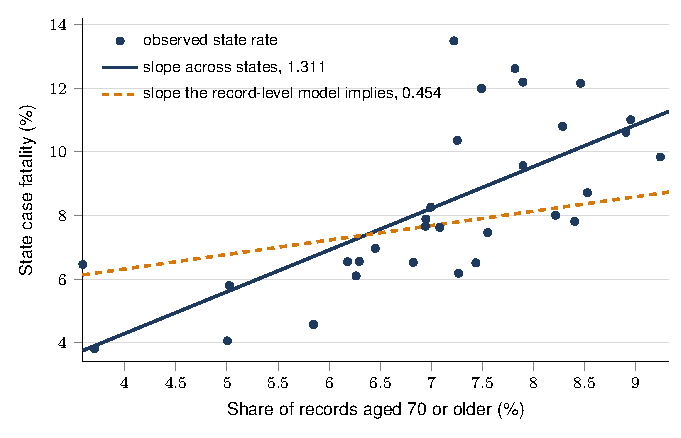
\includegraphics[width=0.92\textwidth]{figures/fig1_two_slopes.pdf}
\caption{Each point is one of Mexico's 32 treating-unit states,
3\,993\,464 confirmed COVID-19 case records.  Points are each state's
observed case fatality.  The solid line is their regression on elderly
share.  The dashed line is the regression, over the same 32 states, of
the rate implied by averaging a record-level logistic model's predicted
probabilities over that state's own patients, under the registered model
carrying age 70 or older, sex and any of nine comorbidities; the implied
rates themselves are not plotted.  The two slopes are therefore
comparable: 1.311 observed against 0.454 implied.  Their difference,
0.857 percentage points of case fatality per point of elderly share, is
the ecological discrepancy.}
\label{fig:slopes}

\raggedright\footnotesize
\noindent\textbf{Alt text:} Scatter plot of 32 Mexican states, with the
share of records aged 70 or older on the horizontal axis and state case
fatality on the vertical axis.  Points are each state's observed case
fatality.  A solid line through them rises steeply, with slope 1.311.  A
dashed line, the slope the record-level model implies for the same
states, is much flatter at 0.454.  The two lines cross near the middle of
the range and diverge toward both ends, so the relationship observed
across states is far steeper than the one the record-level model
implies.
\end{figure}

Sharing coefficients instead reproduces the record-level association
(Table~\ref{tab:estimators}).  Estimators separate by the quantity they
target rather than by whether the fit is one-stage or two-stage: four
common-effect specifications fall between odds ratios $11.26$ and
$11.28$ and three random-effects specifications between $11.73$ and
$11.74$, while the two aligned pairs differ by $0.00015$ and $0.00068$
in the log odds ratio.  Heterogeneity is preserved rather than hidden: per-state
odds ratios run from $7.99$ to $18.09$, $I^2 = 97.4\%$, with a
prediction interval of $8.43$ to $16.32$.

\begin{table}[t]
\centering
\caption{Estimators of the record-level association between age 70 or
older and death, Mexico, 3\,993\,464 records in 32 treating-unit states.
Specifications are grouped by the quantity they target.  Within each
group, the one-stage and two-stage fits differ by less than $0.0007$ in
the log odds ratio; between groups they differ by 4.2\%, which is the
common-effect against random-effects choice and not the one-stage
against two-stage one.}
\label{tab:estimators}
\begin{tabular}{llc}
\toprule
Target & Specification & Odds ratio \\
\midrule
\multicolumn{3}{l}{\emph{Common effect}} \\
& Pooled record level                  & 11.264 \\
& One-stage, state fixed effects       & 11.275 \\
& One-stage, random intercept          & 11.275 \\
& Two-stage, common effect             & 11.276 \\
\midrule
\multicolumn{3}{l}{\emph{Random effects}} \\
& Two-stage, DerSimonian--Laird        & 11.729 \\
& Two-stage, REML, Hartung--Knapp      & 11.737 \\
& One-stage, random slope              & 11.737 \\
\bottomrule
\end{tabular}
\end{table}

\subsection{Dependence on the record-level model}

The discrepancy is defined against a model, and it shrinks as that model
is enriched (Table~\ref{tab:ladder}).  Entering age as a spline with the
nine comorbidities separately moves the implied slope from $+0.4537$ to
$+0.6549$ and the discrepancy from $+0.8568$ to $+0.6557$; adding
calendar month of onset leaves $+0.5941$.  The bootstrap interval
excludes zero at every rung.  A model carrying a free term per state
would reproduce each state's rate exactly and remove the discrepancy
altogether, so the quantity measures state-structured lack of fit of a
specified model rather than a model-free amount of ecological bias.

\begin{table}[t]
\centering
\caption{Observed minus model-implied ecological slope across six
prespecified record-level models, in percentage points of case fatality
per point of elderly share.  The observed slope is $+1.3105$ throughout.
Intervals are a state bootstrap with the record-level model refitted in
each draw.  Specifications were registered at commit \texttt{a38196b}
before any was fitted.}
\label{tab:ladder}
\begin{tabular}{lccc}
\toprule
Record-level model & Implied & Difference & 95\% CI \\
\midrule
Age 70+                                   & 0.332 & 0.979 & 0.605--1.458 \\
\;\;+ sex, any comorbidity \emph{(registered)} & 0.454 & 0.857 & 0.496--1.303 \\
\;\;+ nine comorbidities separately       & 0.495 & 0.816 & 0.477--1.243 \\
\;\;age in ten-year bands instead           & 0.650 & 0.661 & 0.269--1.148 \\
\;\;age as a restricted cubic spline instead & 0.655 & 0.656 & 0.260--1.149 \\
\;\;+ calendar month of onset             & 0.716 & 0.594 & 0.212--1.070 \\
\bottomrule
\end{tabular}
\end{table}

\subsection{Dependence on the site definition}

The discrepancy is also a property of how sites are drawn
(Table~\ref{tab:sites}).  It is $+0.8497$ across the 32 states of
residence and $+0.7657$ across the 11 health-care sectors.  On the
3\,665\,523 records retained by the municipality size rule, it is
$+0.4689$ across 385 municipalities against $+1.0087$ across the states
those municipalities nest in, a paired difference of $-0.5398$
(state-clustered bootstrap $-1.1642$ to $-0.1299$).  The discrepancy is smaller at finer grain, consistent with what is reported for nested residential
geographies \cite{best2001ecological,lancaster2006reducing}, although
elderly share is measured from the same records and is estimated less
precisely in small units.

A registered reassignment of records to pseudo-sites holding each
state's size and elderly count fixed returns a median discrepancy of
$+0.0005$ over 500 replications.  Its expectation is zero by the
estimating equations, so it checks the construction rather than
geography, and the supplement reports it in full.

\begin{table}[t]
\centering
\caption{Observed and model-implied ecological slopes under each
prespecified site definition, with the registered three-covariate
record-level model.  The municipality row is restricted to municipalities
with at least 1000 records and is paired against the states of residence
those municipalities nest in, on the same records.}
\label{tab:sites}
\begin{tabular}{lcccc}
\toprule
Site definition & Sites & Observed & Implied & Difference \\
\midrule
Treating-unit state        & 32  & 1.311 & 0.454 & 0.857 \\
State of residence         & 32  & 1.305 & 0.455 & 0.850 \\
Health-care sector         & 11  & 1.193 & 0.428 & 0.766 \\
Municipality ($\geq$1000 records) & 385 & ---   & ---   & 0.469 \\
\;\;paired states of residence    & 32  & ---   & ---   & 1.009 \\
\bottomrule
\end{tabular}
\end{table}

\subsection{A residual state-level association}

Fitting the state's standardized elderly share alongside the
record-level covariates of the richest composition model, as a binomial
random-intercept model over 152\,919 cells by adaptive Gauss--Hermite
quadrature at 15 nodes, leaves an odds ratio of $1.1817$ per standard
deviation (profile-likelihood interval $1.0719$ to $1.3027$) with a
random-intercept standard deviation of $0.2682$.  The fit meets all
eleven numerical acceptance criteria fixed before it was run, and a
second implementation of the same quadrature, written separately and
run on the same cells, reproduces its coefficients to
$7.7\times10^{-5}$.  The association is estimated from 32 clusters and conditions
on the measured record-level covariates only, so it is a model-based
residual association and not an identified contextual effect.

\section{Discussion}
\label{sec:discussion}

\subsection{What the difference contains}
\label{sec:why}

A regression across site rates absorbs any between-site variation in the
outcome that correlates with the regressor, whatever produces it.  The
slope implied by a record-level model includes only what that model
attributes to the covariates it holds, averaged over each site's own
covariate distribution.  Their difference is therefore the component
of what the site rates contain, aligned with elderly share, that the
record-level model does not reproduce, and
the covariate ladder bounds it from one side, showing that measured
composition accounts for part of it and leaves the rest.

What remains is not attributable from this design.  It contains
unmeasured composition, differences in case ascertainment and coding
between states, the point each state had reached in its epidemic, any
genuine effect of where a patient was treated, and misspecification of
the record-level model, which enters the residual by construction.
Noncollapsibility of the odds ratio
\cite{greenland1999noncollapsibility} does not contaminate the
comparison, because the implied slope is formed from predicted
probabilities rather than from a conditional coefficient; it does bear
on any attempt to read the record-level odds ratio as the quantity the
ecological slope is estimating.

Nothing in the comparison is specific to COVID-19.  COVID-19 serves
here because the available record-level data permit both halves of the
comparison on the same cohort; the same structure applies to drug-safety
surveillance, federated genomic association, and any multi-site study
pooling site-level summaries.

\subsection{Implications for federated analysis infrastructure}

A network that shares site rates and a network that shares per-site
coefficients are not doing the same analysis at different levels of
privacy.  The rate regression estimates a relationship between
site-level quantities; the coefficient estimates a within-site
association among records.  On these data the second is recoverable from
shared summaries to within $0.0007$ in the log odds ratio, and the
first includes an additional $+0.8568$ that no record-level model we
registered reproduces.  Which object a network shares therefore
determines what its central analysis can estimate, and the choice is an
estimand question before it is a privacy or engineering one.

That does not make rate sharing wrong.  A cross-site rate relationship
is a well-defined quantity and may be the one a surveillance question
asks for.  It is wrong only when read as the association among patients,
and a network cannot tell the two apart from site rates alone: the
discrepancy is invisible from those marginal summaries.  Four
routes avoid the substitution.

\textbf{Joint stratum counts.}  Every covariate in the specifications
reported here takes finitely many values, so the record-level fit, the
model-implied slope and the discrepancy are computable from counts of
deaths and records in each joint stratum of age, sex, comorbidity and
month within each site; the state-level model is fitted over
152\,919 such cells.  A coordinating center that receives joint counts
rather than marginal rates can compute the benchmark without individual
records.  Joint counts remain potentially disclosive because a fine
stratum may contain one person; minimum cell sizes, suppression, or
other network-appropriate disclosure controls are still required.

\textbf{Federated regression.}
Fed-GLMM~\cite{yan2023fedglmm} and
DataSHIELD~\cite{banerjee2022dssurvival} enable record-level estimation
while sharing only summary statistics: sites run a standardized script
locally and share coefficients, supporting record-level estimation
without the aggregation substitution studied here.

\textbf{Large individual-level cohorts.}  N3C~\cite{haendel2021n3c} holds individual
records for direct estimation across more than 75 sites.

\textbf{Hierarchical models.}  Multilevel models with site random
effects represent both levels explicitly rather than choosing one
\cite{diezroux2000multilevel}, and shrinkage toward the group mean
limits the inflation of extreme site-level estimates
\cite{gelman2012multilevel}.

\subsection{Practical guidelines for multi-site studies}

\paragraph{Name the estimand the shared object supports.}
A protocol that says a network will ``pool site-level data'' has not
said what it will estimate.  Site rates support a cross-site
relationship; per-site coefficients support a within-site association.
Writing which one the study targets, before the summaries are
collected, is the step that makes the rest checkable.

\paragraph{Report heterogeneity rather than averaging it away.}
A pooled odds ratio of 11.73 is the right answer to the question it
answers; the prediction interval of 8.43 to 16.32 is what tells a
reader whether that is the question they have.

\paragraph{Share coefficients when the target is a record-level
association.}  The agreement in Table~\ref{tab:estimators} holds for
compatible local models, harmonized coding and adequate cell counts at
each site.  A network has to verify those rather than assume them.

\paragraph{Register the benchmark, not only the procedure.}
Where a reported quantity is a comparison against a model, the model is
part of what is being reported.  The discrepancy here moves from
$+0.979$ to $+0.594$ across six record-level specifications.  Weighting
moves it further, from $+0.857$ under equal-state fitting to $+1.322$
under record-count fitting, and that movement reflects a change in the
target relationship, not instability of a single estimate.
A registration that fixes the procedure and leaves the benchmark and
the weighting open has not fixed the number.

\section{Limitations}

\textbf{No specification is established as correct.}  The discrepancy
is the part of the cross-site rate relationship a given record-level
model does not reproduce, so a better model would leave less of it and
a model with a free term per state would leave none.  The paper reports
the range across six registered specifications and does not identify a
true one.

\textbf{A discrepancy near zero does not certify the site
predictions.}  The statistic is the association between elderly share
and the aggregated residual, so it captures only the component of
site-level error aligned with that share.  Three equally weighted sites
with equally spaced elderly shares and residuals of $+5$, $-10$ and
$+5$ percentage points give a residual slope of exactly zero: the equal
endpoint errors cancel in the slope, while the middle error falls at
the mean elderly share.

\textbf{The residual is not attributable.}  This design cannot
separate the sources enumerated in Section~\ref{sec:discussion}.

\textbf{The diagnostic is not evaluated as a guide to action.}
Whether acting on a nonzero discrepancy improves later predictions is a
separate question from whether the discrepancy is present, and these
analyses do not test that use.  Answering it requires temporally
separated evaluation against ordinary recalibration.

\textbf{Finer units are measured less precisely.}  Elderly share is
estimated from the same records, so the municipality comparison
confounds geographic grain with measurement error in the regressor.  The
grouped-binomial fit reported beside the equal-state one addresses
outcome variance in small municipalities, not error in the regressor,
which nothing here corrects.

\textbf{The architectures are reproduced, not observed.}  A live
network differs in local model specification, coding harmonization and
per-site cell counts, and the agreement between pooling strategies
reported here is conditional on those being adequate.  The source
carries record identifiers and no person identifiers, so repeat
presentations by one patient are counted separately.

\section{Conclusion}

A network that shares site rates cannot find this discrepancy in what it
shares.  The observed slope and its interval are computable from the
rates; the benchmark they would have to be set against is not, because
forming it requires the joint distribution of the covariates within
each site.  Nothing in the shared rates indicates whether the gap is
0.86 or zero, and the joint counts that would carry it are a different
summary rather than the records themselves.

The choice of shared object therefore has to be made when a network is
designed, from the estimand the study will report, and cannot be
audited afterward from the summaries it produced.  Where the target is
an association among patients, per-site coefficients from aligned local
models carry it; where the target is a relationship between sites,
rates carry that, and the two should not be read as estimates of each
other.

\section{Supplementary Materials}
\label{app:supplementary}

Available online:
(A)~the two frozen protocols, the implementation amendments and the
correction record, with a provenance table giving for each analysis its
status, what was known when it was specified, and the commit that froze
it;
(B)~an accounting table reconciling every denominator the paper uses,
and a table of superseded values with the cause of each;
(C)~the ten registered supplementary analyses with their falsification
criteria and outcomes, reported regardless of result;
(D)~per-state estimates, the binomial and record-count-weighted
sensitivities beside the equal-state primary fit, and the municipality
analysis at all four registered size thresholds;
(E)~the full numerical diagnostics for the state-level model, including
the second implementation and the eleven acceptance criteria;
(F)~two further record sets analyzed under the same design, United
States case surveillance grouped by race and ethnicity and the 4CE
consortium's aggregate neurological data, which are not part of the
analysis reported here.

\section*{Declarations}

\subsection*{Ethics approval and consent to participate}
This study used only publicly available, de-identified datasets.  No
ethics approval or informed consent was required.  The CDC Case
Surveillance Public Use Dataset is released under a public domain license.
The Mexico Datos Abiertos dataset is released by the Secretar\'{i}a de
Salud for public use.  The United States and 4CE data appear only in the
supplement; the 4CE material is the aggregate site-level summaries
published in \cite{four_ce_neuro2021}.

\subsection*{Consent for publication}
Not applicable.

\subsection*{Availability of data and materials}
The Mexico COVID-19 surveillance data is available from
\texttt{datos.gob.mx} \cite{dataset_mexico_covid}, and the CDC COVID-19
Case Surveillance Public Use Dataset from \texttt{data.cdc.gov}
\cite{dataset_cdc_covid}.  The 4CE aggregate data is available in the supplementary
materials of \cite{four_ce_neuro2021}.  Neither the CDC nor the 4CE
records are part of the analysis reported here; both are described in
the supplement.  All analysis code, the frozen
pre-registration protocol, and computed results are available at
\url{https://github.com/elliottower/ecological-bias-covid}.
A permanent archive is deposited at Zenodo
(DOI: 10.5281/zenodo.21252372).

\subsection*{Competing interests}
The author declares no competing interests.

\subsection*{Funding}
This research received no specific grant from any funding agency in the
public, commercial, or not-for-profit sectors.

\subsection*{Authors' contributions}
ET conceived the study, designed the analyses, wrote the code, performed
all statistical analyses, and wrote the manuscript.  The author read and
approved the final manuscript.

\subsection*{Acknowledgements}
The research question, the two pre-registration protocols, the choice of
specifications and site definitions, and all interpretations are the
author's.  Claude Code (Anthropic, versions 2.1.220 to 2.1.287, running
the models Claude Opus 4.6, Claude Opus 5 and Claude Opus 5.5) was used
between July and October 2026 to draft and edit manuscript text and to
write and debug the analysis code.  Perplexity AI (web application) was
used for literature search and to review near-final drafts.  The author
directed and reviewed all of that work, verified every reported number
against the record that produced it, and takes full responsibility for
the accuracy and integrity of the work.  No AI tool is listed as an
author, and no AI-generated content was used as a primary data source.

\bibliographystyle{vancouver-jamia}
\bibliography{references}

\end{document}
